
\usepackage{tikz} 
\usepackage{mathptmx}
%\usepackage[T1]{fontenc}
\usepackage[latin1]{inputenc}
\usepackage{color}
\usepackage{amsmath}
\usepackage{amssymb}


%%%%%%%%%% Farseerfc: fix the bug of xetex on navigation bar of beamer %%%%%%%%%

\def\beamer@linkspace#1{%
  \begin{pgfpicture}{0pt}{-1.5pt}{#1}{5.5pt}
    \pgfsetfillopacity{0}
    \pgftext[x=0pt,y=-1.5pt]{.}
    \pgftext[x=#1,y=5.5pt]{.}
  \end{pgfpicture}}

%%%%%%%%%% Farseerfc: fix the bug of xetex on navigation bar of beamer %%%%%%%%%

\usetheme{Warsaw}
\usecolortheme[named=OliveGreen]{structure}
%\setbeamercovered{dynamic}
\useoutertheme{infolines}
\usepackage[english]{babel}


\graphicspath{{figure/}}
\begin{document}

%%%%%%%%%%%%%%%%%%%%%%%%%%%%%%%%%%%%%%%%%%%%%%%%%%%%%%%%%%%%%%%%%%%%%%%%%%%%%%%%
% Farseerfc defined commands

\newcommand{\br}[0]{\par\vskip15pt\par}
%\newenvironment{topcolumns}{\begin{columns}[t]}{\end{columns}}

%%%%%%%%%%%%%%%%%%%%%%%%%%%%%%%%%%%%%%%%%%%%%%%%%%%%%%%%%%%%%%%%%%%%%%%%%%%%%%%%



\title[SuffixTree]{Algorithm of Suffix Tree Construction}

\subtitle{by farseerfc@gmail.com}

\author[jc-yang]{
	Jiachen Yang\inst{1} 
}

\institute[Osaka-U]{
	\inst{1}Research Student in Osaka University
}



\frame{\maketitle}


\AtBeginSubsection[]{
  \frame<beamer>{ 
    \frametitle{Section Outline}   
    \tableofcontents[currentsection,currentsubsection] 
  }
}

\AtBeginSection[]{
  \frame<beamer>{ 
    \frametitle{Part Outline}   
    \tableofcontents[currentpart,currentsection] 
  }
}

\AtBeginPart{
  \frame<beamer>{
	\partpage
  }
}

%%%%%%%%%%%%%%%%%%%%%%%%%%%%%%%%%%%%%%%%%%%%%%%%%%%%%%%%%%%%%%%%%%%%%%%%%%%%%%%%
\section{What I did} 

\begin{frame}{Algorithm of Constructing Suffix Tree}%
\begin{columns}%
\transdissolve[duration=0.2]<2->
\column{0.5\textwidth}
\includegraphics[width=\textwidth]{mississippi.pdf}

\column{0.45\textwidth}
\begin{itemize}
\item<2-> 
\includegraphics[width=0.25\textwidth,trim=40pt 40pt 40pt 40pt]{gray.pdf} 
Node (id:generation)
\item<3-> 
\includegraphics[width=0.25\textwidth,trim=40pt 40pt 40pt 40pt]{box.pdf} 
Leaf
\item<4-> 
\includegraphics[width=0.25\textwidth,trim=40pt 40pt 40pt 40pt]{line.pdf} 
Child-relation
\item<5-> 
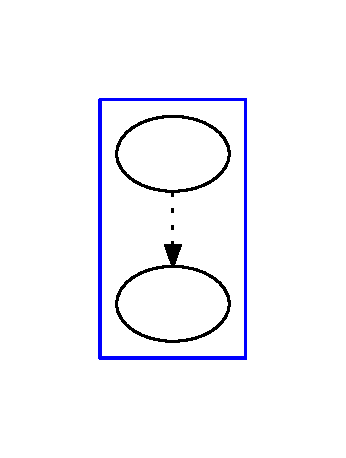
\includegraphics[width=0.25\textwidth,trim=40pt 40pt 40pt 40pt]{dotted.pdf} 
suffix-link relation
\end{itemize}
\end{columns}
\end{frame}

%%%%%%%%%%%%%%%%%%%%%%%%%%%%%%%%%%%%%%%%%%%%%%%%%%%%%%%%%%%%%%%%%%%%%%%%%%%%%%%%
\begin{frame}{Experiment -- mississippi}

\transdissolve[duration=0.1]<2->
\begin{overlayarea}{\textwidth}{\textheight}
\includegraphics[keepaspectratio,height=0.9\textheight,width=0.9\textwidth]{m.pdf}<1>
\includegraphics[keepaspectratio,height=0.9\textheight,width=0.9\textwidth]{mi.pdf}<2>
\includegraphics[keepaspectratio,height=0.9\textheight,width=0.9\textwidth]{mis.pdf}<3>
\includegraphics[keepaspectratio,height=0.9\textheight,width=0.9\textwidth]{miss.pdf}<4>
\includegraphics[keepaspectratio,height=0.9\textheight,width=0.9\textwidth]{missi.pdf}<5>
\includegraphics[keepaspectratio,height=0.9\textheight,width=0.9\textwidth]{missis.pdf}<6>
\includegraphics[keepaspectratio,height=0.9\textheight,width=0.9\textwidth]{mississ.pdf}<7>
\includegraphics[keepaspectratio,height=0.9\textheight,width=0.9\textwidth]{mississi.pdf}<8>
\includegraphics[keepaspectratio,height=0.9\textheight,width=0.9\textwidth]{mississip.pdf}<9>
\includegraphics[keepaspectratio,height=0.9\textheight,width=0.9\textwidth]{mississipp.pdf}<10>
\includegraphics[keepaspectratio,height=0.9\textheight,width=0.9\textwidth]{mississippi.pdf}<11>
\includegraphics[keepaspectratio,height=0.9\textheight,width=0.9\textwidth]{mississippi_.pdf}<12>
\end{overlayarea}
\end{frame}
%%%%%%%%%%%%%%%%%%%%%%%%%%%%%%%%%%%%%%%%%%%%%%%%%%%%%%%%%%%%%%%%%%%%%%%%%%%%%%%%
\begin{frame}{Experiment -- English text}

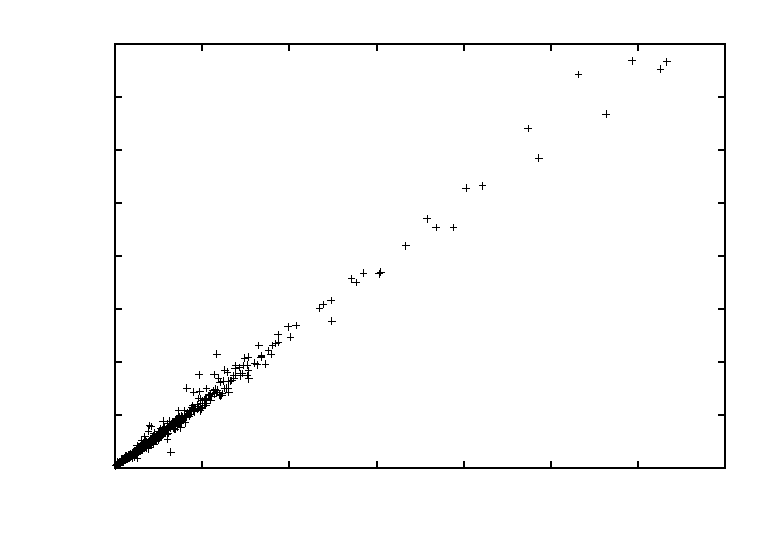
\includegraphics[angle=270,width=0.9\textwidth]{plot.ps}
\end{frame}
%%%%%%%%%%%%%%%%%%%%%%%%%%%%%%%%%%%%%%%%%%%%%%%%%%%%%%%%%%%%%%%%%%%%%%%%%%%%%%%%
\section{Future works}
\begin{frame}{Works in next week}
\transwipe[direction=270]
\begin{itemize}[<+->]
\item Implementing \alert{Longest Common Substring} algorithm using
\alert{Generalised Suffix Tree} based on Ukk's algorithm.
\item Implementing \alert{Tokenization} on Python codes.
\item Implementing \alert{DC3} algorithm of \alert{Suffix Array} and compare
their performance.
\item Reading and Understanding \alert{n-gram} algorithm and its
application in code-clone detectation.
\end{itemize}
\end{frame}
\end{document}
